% --------------------------------------------------------------------------------

\begin{exercise}[Exercise 2.6 Mysterious Spikes]

The results shown in Figure \ref{fig:1.6} (below) should be quite reliable because they are averages over $2000$ individual, randomly chosen $10$-armed bandit tasks.
Why, then, are there oscillations and spikes in the early part of the curve for the optimistic method?
In other words, what might make this method perform particularly better or worse, on average, on particular early steps?

\begin{figure}[H]
    \centering
    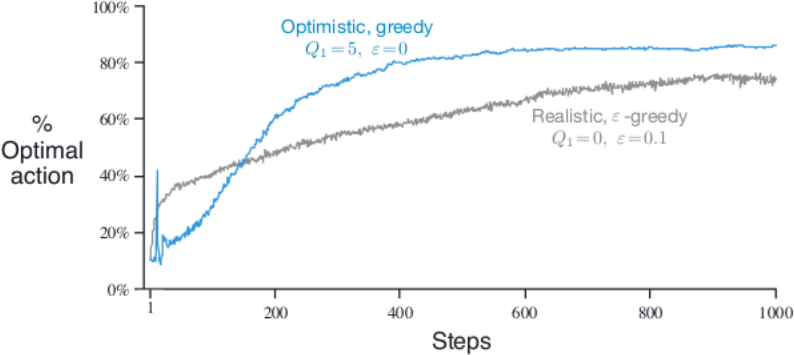
\includegraphics[width = 0.5 \textwidth]{1.6.png}
    \caption
    {
        The effect of optimistic initial action-value estimates on the $10$-armed testbed.
        Both methods used a constant step-size parameter, $\alpha = 0.1$.
    }
    \label{fig:1.6}
\end{figure}

\end{exercise}

% --------------------------------------------------------------------------------

\begin{solution}

At first, the estimated expected rewards $Q_1 = 5$.
Since $q_\ast \sim N(0, 1)$ and $R \sim N(q_\ast, 1)$, in order for $R$ to yield a reward $\approx 5$, it would have to stray (twice) $5$ standard deviations in total from the initial mean $0$.
This is wildly unrealistic!
Hence, at first the estimated expected rewards $Q_2, \dots$ get lowered via \eqref{eq} with $\alpha = 0.1$.

The amount by which $Q(a)$, for $a = 1, \dots, 10$ gets lowered (towards $q_\ast(a)$) $\alpha (R - Q)$ roughly depends on how low $q_\ast$ is (because of $R$).
Thus, for the optimal action $a_\text{opt} = \argmax_{a=1}^{10} q_\ast(a)$, $Q(a_\text{opt})$ would not get lowered as quickly as for other actions.
Therefore, it must be selected more often, in order for $Q(a_\text{opt})$ to get squished towards $q_\ast(a_\text{opt})$.

\end{solution}

% --------------------------------------------------------------------------------
